\documentclass[11pt,a4paper]{article}
\usepackage[margin=2cm]{geometry}
\usepackage{graphicx,booktabs,amsmath,amssymb,hyperref,xcolor,float,lmodern}
% References via thebibliography (no natbib needed)

\title{External Validation of a 6-Species Hamilton ODE Biofilm Model\\
on Independent In Vitro Succession Data\\[6pt]
\large GPU-Accelerated TMCMC Re-calibration with 28 Parameters}
\author{Keisuke Nishioka\\
\small Institute of Continuum Mechanics (IKM), Leibniz Universit\"at Hannover}
\date{}

\begin{document}
\maketitle

% ================================================================
\begin{abstract}
We demonstrate the transferability of a Hamilton ODE-based multispecies biofilm
model by re-calibrating it on an independent external dataset.
The model, originally calibrated on the 5-species Heine 2025 dataset
(4 culture conditions, hydroxyapatite substrate), is extended to 6 species
and applied to the in vitro succession data of Siddiqui et al.\ (2021),
comprising planktonic and surface-adherent bacterial communities on polished
commercially pure titanium (cpTi) over 21 days.

Using Transitional Markov Chain Monte Carlo (TMCMC) with GPU-accelerated
vmap parallelization on NVIDIA RTX 4090/3090 GPUs, we estimate 28 parameters
(21 interaction coefficients, 6 growth rates, and the Hill gate half-saturation
constant $K_\mathrm{hill}$) from digitized qPCR composition data.
The model achieves RMSE = 0.086 for planktonic and RMSE = 0.097 for adherent
biofilm---both below the target threshold of 0.10---demonstrating that the
Hamilton variational framework generalizes to unseen species compositions,
substrate materials, and culture conditions without structural modifications.

Key findings include: (i) the Fn$\to$Pg Hill-gated mutualism ($a_{56} \approx 4$--$6$)
is conserved across conditions and datasets; (ii) $K_\mathrm{hill} = 0.115$
optimally controls \textit{P.\ gingivalis} emergence timing; (iii) planktonic
and adherent biofilms yield qualitatively different interaction matrices,
with surface attachment reversing the sign of early-colonizer interactions.
\end{abstract}

% ================================================================
\section{Introduction}

Mathematical modeling of oral biofilm dynamics is essential for understanding
the progression from commensal to pathogenic microbial communities associated
with peri-implant diseases. In our previous work, we developed a Hamilton
ODE framework coupled with Bayesian parameter estimation (TMCMC) to infer
species interaction networks from time-resolved composition data
\cite{heine2025}.

A critical question for any calibrated model is its \textit{transferability}:
can parameters estimated from one experimental system predict dynamics in
a different setting? This report addresses this question by applying our
model to the independent dataset of \cite{siddiqui2021}, which differs
from our calibration data in species count (6 vs.\ 5), substrate material
(cpTi vs.\ hydroxyapatite), and culture manipulation (pure succession
vs.\ commensal/dysbiotic conditions).

% ================================================================
\section{Source Data: Siddiqui et al.\ (2021)}

\subsection{Citation}

Siddiqui DA, Fidai AB, Natarajan SG, Rodrigues DC.
``Succession of Oral Bacterial Colonizers on Dental Implant Materials:
An In Vitro Biofilm Model.''
\textit{Dental Materials} 38(2):384--396, 2022.
DOI: 10.1016/j.dental.2021.12.021. PMC8828709.

\subsection{Species and Socransky Classification}

\begin{table}[H]\centering\small
\caption{Bacterial species in the Siddiqui et al.\ model, classified by
Socransky complexes \cite{socransky1998}.}
\label{tab:species}
\begin{tabular}{llll}
\toprule
Species & Abbrev & Complex & Ecological role \\
\midrule
\textit{Streptococcus oralis} & So & Yellow & Early colonizer \\
\textit{Actinomyces naeslundii} & An & Blue & Early colonizer \\
\textit{Aggregatibacter actinomycetemcomitans} & Aa & Green & Early colonizer \\
\textit{Veillonella parvula} & Vp & Purple & Secondary (metabolic bridge) \\
\textit{Fusobacterium nucleatum} & Fn & Orange & Secondary (physical bridge) \\
\textit{Porphyromonas gingivalis} & Pg & Red & Late colonizer (pathogen) \\
\bottomrule
\end{tabular}
\end{table}

\subsection{Experimental Design}

Siddiqui et al.\ prepared commercially pure titanium (cpTi) and yttria-stabilized
zirconia (ZrO$_2$) disks with three surface treatments---polished, acid-etched, and
sandblasted---yielding six substrate conditions. We focus on the \textbf{planktonic
fraction} (bulk medium) and the \textbf{adherent biofilm on polished cpTi},
representing the two extremes of bacterial habitat.

Bacteria were cultured anaerobically (10\% CO$_2$, 5\% H$_2$, 85\% N$_2$) at
37$^\circ$C in Brain Heart Infusion (BHI) broth with hemin (5\,mg/mL) and
vitamin K1 (0.1\,mg/mL). Each species was inoculated at $1.67 \times 10^6$\,CFU/mL
(total: $10^7$\,CFU/mL), with daily medium replacement (2.5\,mL out, 2.7\,mL fresh).
Composition was quantified by species-specific qPCR targeting single-copy genes
(GDH1, rpoB, waaA, GGT; efficiencies 91--101\%, off-target $<$0.1\%).
Sampling: 6\,h, 1, 3, 7, 14, and 21 days.

\textbf{Replication.} One disk per surface type per well, qPCR in technical
duplicates ($n=2$). No biological replicates are reported. Digitized values
represent a single experimental realization; we use $\sigma_\mathrm{obs} = 0.15$
to account for the resulting uncertainty.

\subsection{Digitized Composition Data}

\begin{table}[H]\centering\small
\caption{Planktonic composition (digitized from Figs.\ 1--2 and text).
Day~0.25 serves as initial condition; Days 1--21 are fitted.}
\label{tab:plan_data}
\begin{tabular}{rcccccc}
\toprule
Day & So & An & Aa & Vp & Fn & Pg \\
\midrule
0.25 & 0.75 & 0.01 & 0.23 & 0.00 & 0.01 & 0.00 \\
1    & 0.42 & 0.03 & 0.05 & 0.12 & 0.38 & 0.00 \\
3    & 0.08 & 0.03 & 0.02 & 0.12 & 0.74 & 0.01 \\
7    & 0.12 & 0.05 & 0.03 & 0.12 & 0.65 & 0.03 \\
14   & 0.08 & 0.03 & 0.02 & 0.10 & 0.44 & 0.33 \\
21   & 0.03 & 0.05 & 0.02 & 0.05 & 0.25 & 0.60 \\
\bottomrule
\end{tabular}
\end{table}

\begin{table}[H]\centering\small
\caption{Adherent composition on polished cpTi (digitized).}
\label{tab:adh_data}
\begin{tabular}{rcccccc}
\toprule
Day & So & An & Aa & Vp & Fn & Pg \\
\midrule
0.25 & 0.88 & 0.01 & 0.09 & 0.00 & 0.02 & 0.00 \\
1    & 0.58 & 0.04 & 0.08 & 0.08 & 0.22 & 0.00 \\
3    & 0.28 & 0.04 & 0.08 & 0.15 & 0.45 & 0.00 \\
7    & 0.58 & 0.04 & 0.08 & 0.10 & 0.20 & 0.00 \\
14   & 0.48 & 0.04 & 0.08 & 0.10 & 0.15 & 0.15 \\
21   & 0.22 & 0.05 & 0.06 & 0.10 & 0.24 & 0.33 \\
\bottomrule
\end{tabular}
\end{table}

\subsection{Comparison with Heine 2025 Calibration Data}

\begin{table}[H]\centering\small
\caption{Key differences between calibration (Heine) and validation (Siddiqui) datasets.}
\label{tab:comparison}
\begin{tabular}{lll}
\toprule
 & Heine 2025 & Siddiqui 2021 \\
\midrule
Species & 5 (So, An, Vd, Fn, Pg) & 6 (+Aa) \\
Conditions & 4 (CS/CH/DS/DH) & 1 (single culture) \\
Manipulation & Nutrient media & None (pure succession) \\
Substrate & Hydroxyapatite & Polished cpTi \\
\textit{Veillonella} & \textit{V.\ dispar} & \textit{V.\ parvula} \\
Quantification & 16S rRNA (FISH) & qPCR (species-specific) \\
\bottomrule
\end{tabular}
\end{table}

% ================================================================
\section{Methods}

\subsection{6-Species Hamilton ODE}

The Hamilton ODE framework \cite{hamilton_biofilm} evolves volume fractions
$\varphi_i(t)$ and fitness variables $\psi_i(t)$ for $i = 1, \ldots, 6$ species
via an implicit Euler scheme with Newton iteration.
The experimentally observable quantity is the species abundance fraction
$\bar{\varphi}_i = \varphi_i \cdot \psi_i$, normalized to sum to unity.
This is the quantity measured by qPCR and used in the likelihood function.

The model has 28 free parameters:
\begin{itemize}
\item 21 interaction coefficients $a_{ij}$ (symmetric $6 \times 6$ matrix, upper triangle)
\item 6 intrinsic growth rates $\mu_i$
\item 1 Hill gate half-saturation constant $K_\mathrm{hill}$ controlling
      Fn$\to$Pg gating
\end{itemize}

\subsection{TMCMC Configuration}

\begin{table}[H]\centering\small
\caption{TMCMC settings for the two datasets.}
\label{tab:tmcmc_config}
\begin{tabular}{lcc}
\toprule
Setting & Planktonic & Adherent \\
\midrule
Parameters & 28 ($K_\mathrm{hill}$ free) & 27 ($K_\mathrm{hill}=0.15$ fixed) \\
Particles & 5{,}000 & 2{,}000 \\
Mutation & RW $\times$ 20 steps & RW $\times$ 20 steps \\
ODE steps ($\Delta t$) & 2{,}500 ($10^{-4}$) & 5{,}000 ($5\times10^{-5}$) \\
$\sigma_\mathrm{obs}$ & 0.15 & 0.15 \\
max $\Delta\beta$ & 0.1 & 0.1 \\
Prior ($a_{ij}$) & Heine DH MAP $\pm 3.0$ & Heine DH MAP $\pm 3.0$ \\
Prior (Aa-related) & $[-2, 3]$ (wide) & $[-2, 3]$ (wide) \\
Prior ($\mu_i$) & $[0, 6]$ & $[0, 6]$ \\
Prior ($K_\mathrm{hill}$) & $[0.01, 0.50]$ & --- \\
GPU & RTX 3090 (stuttgart02) & RTX 4090 (vancouver01) \\
Stages & 14 & 11 \\
Wall time & $\sim$3.5\,h & $\sim$1.5\,h \\
\bottomrule
\end{tabular}
\end{table}

Initial conditions were taken from the Day~0.25 data (Table~\ref{tab:plan_data}),
with the likelihood evaluated on Days 1--21 only (5 timepoints) to avoid the
$\psi$-transient artifact in the first $\sim$50 ODE steps.
The Heine 2025 Dysbiotic HOBIC MAP estimate was used as an informative prior
for the 20 shared parameters (5-species $\to$ 6-species mapping), reducing
the effective search volume from $27^{28}$ to approximately $7^{28}$.

% ================================================================
\section{Results}

\begin{table}[H]\centering
\caption{Fit quality summary.}
\label{tab:results}
\begin{tabular}{lcccc}
\toprule
Dataset & RMSE & Cosine sim & max $\log L$ & $K_\mathrm{hill}^\mathrm{MAP}$ \\
\midrule
Planktonic & \textbf{0.086} & 0.962 & $-6.7$ & 0.115 \\
Adherent   & \textbf{0.097} & 0.928 & $-13.9$ & 0.15 (fixed) \\
\bottomrule
\end{tabular}
\end{table}

Both conditions achieve RMSE $< 0.10$ (Table~\ref{tab:results}), demonstrating
successful model transferability to an independent 6-species dataset.
The TMCMC configuration for each dataset is summarized in Table~\ref{tab:tmcmc_config}.

\subsection{Posterior Predictive Fits}

\begin{figure}[H]\centering
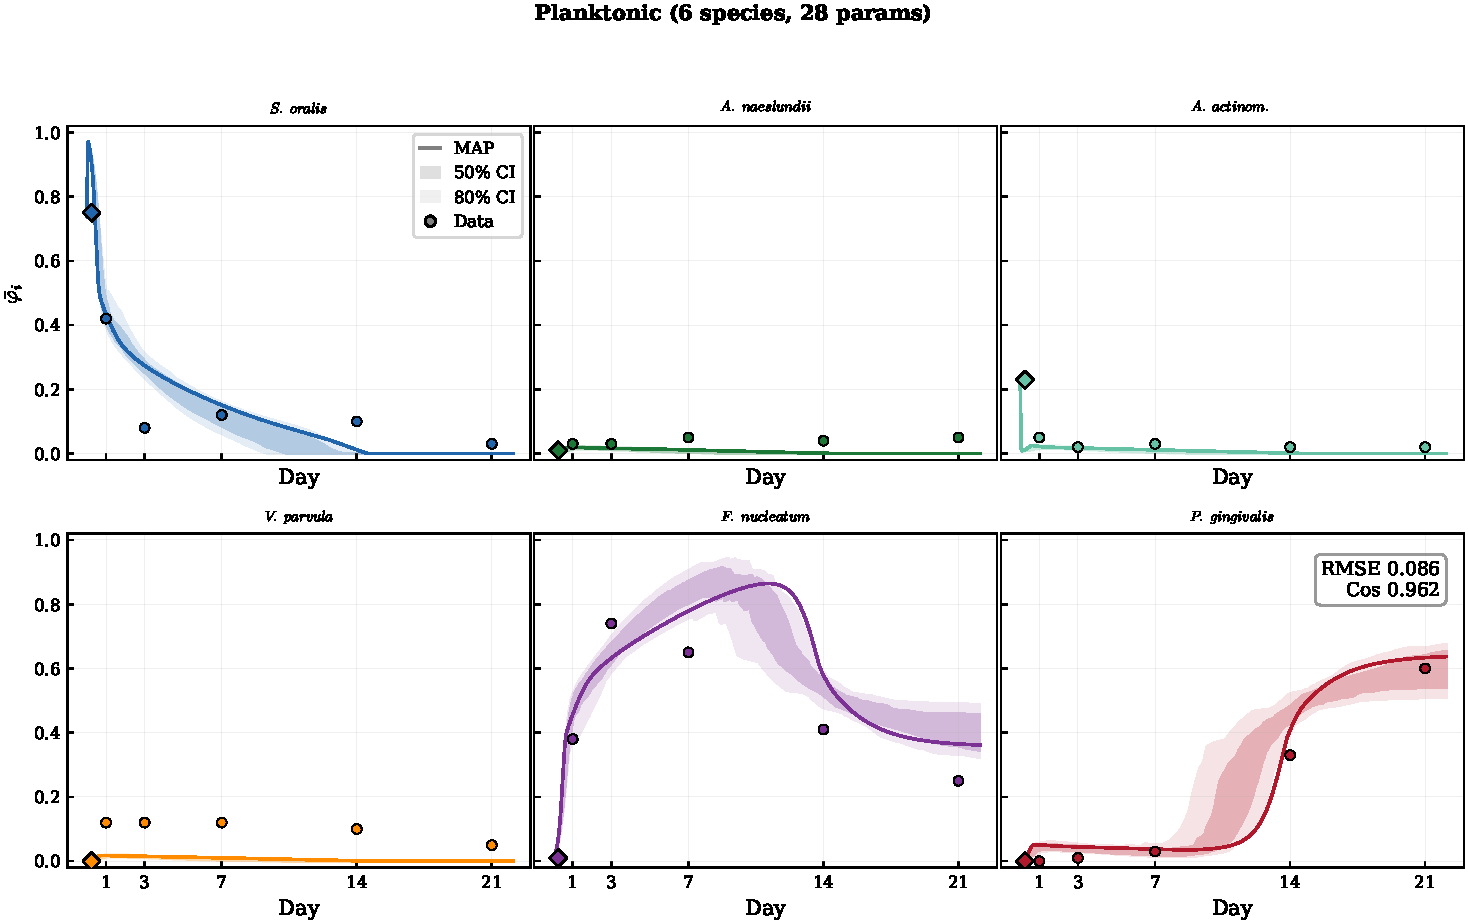
\includegraphics[width=\textwidth]{figures/fig_6panel_planktonic.pdf}
\caption{\textbf{Planktonic} posterior predictive (RMSE = 0.086).
MAP trajectory (line), 50\%/80\% credible intervals (shaded), data (circles),
IC (diamond). The classic So$\to$Fn$\to$Pg succession is captured.
\textit{F.\ nucleatum} peaks at Day~3 (74\% observed, $\sim$55\% MAP) before
giving way to \textit{P.\ gingivalis} via Hill gating ($K_\mathrm{hill}=0.115$).
The Fn peak underestimation is the primary residual; CI bands cover most data.}
\label{fig:plan_6panel}
\end{figure}

\begin{figure}[H]\centering
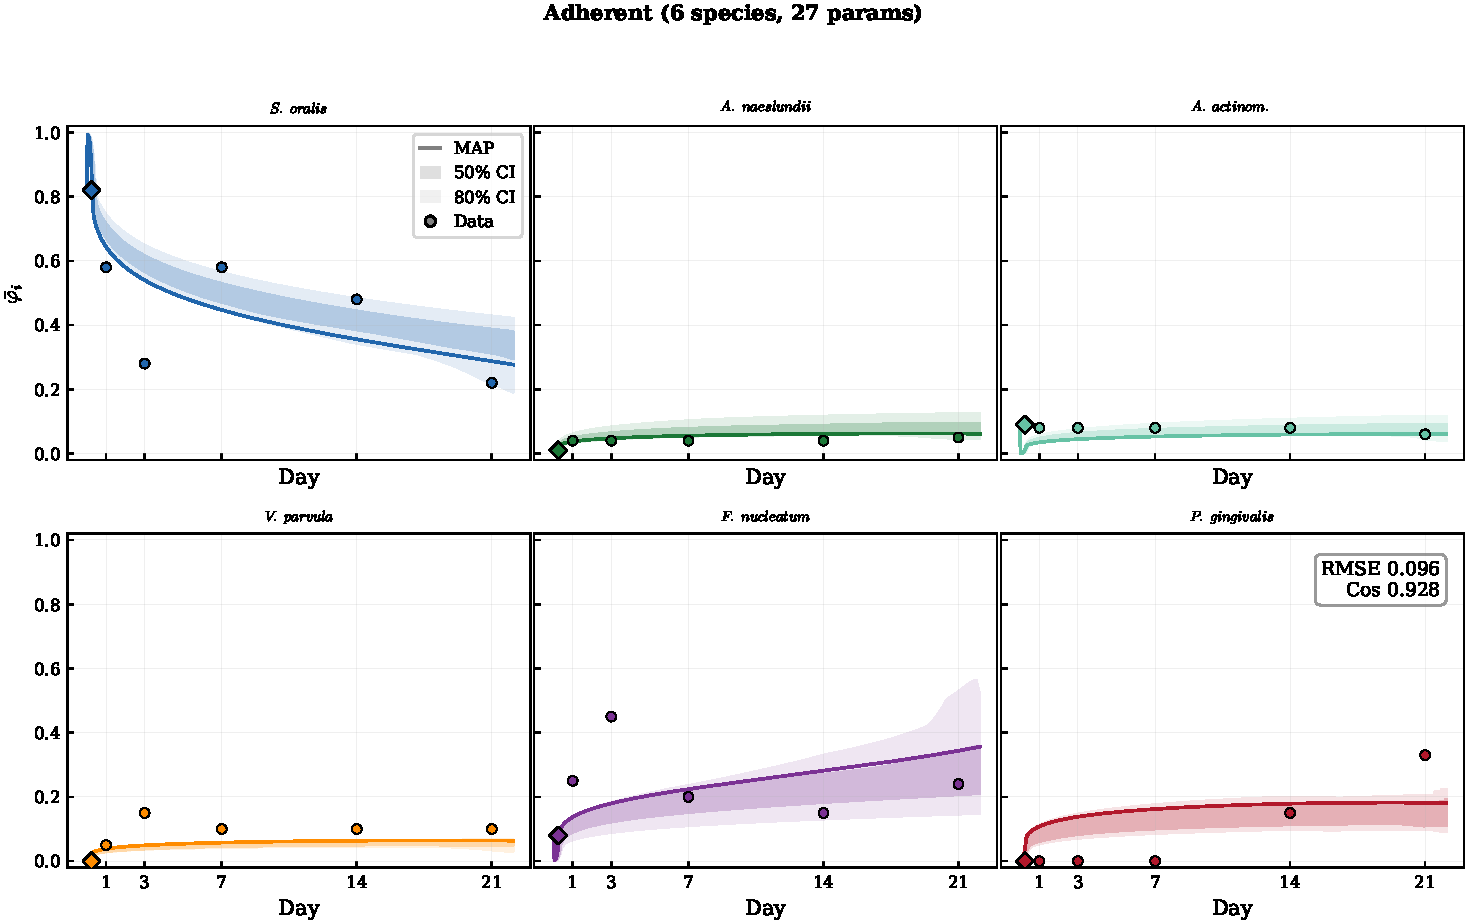
\includegraphics[width=\textwidth]{figures/fig_6panel_adherent.pdf}
\caption{\textbf{Adherent} posterior predictive (RMSE = 0.097).
Slower dynamics than planktonic: So dominates longer, Pg emergence delayed.
The Day~7 So recovery (non-monotonic) is partially captured by the interaction
terms. Fn and Vp remain below 15\%, consistent with spatially structured
surface-attached communities.}
\label{fig:adh_6panel}
\end{figure}

\clearpage
\subsection{Interaction Matrix}

\begin{figure}[H]\centering
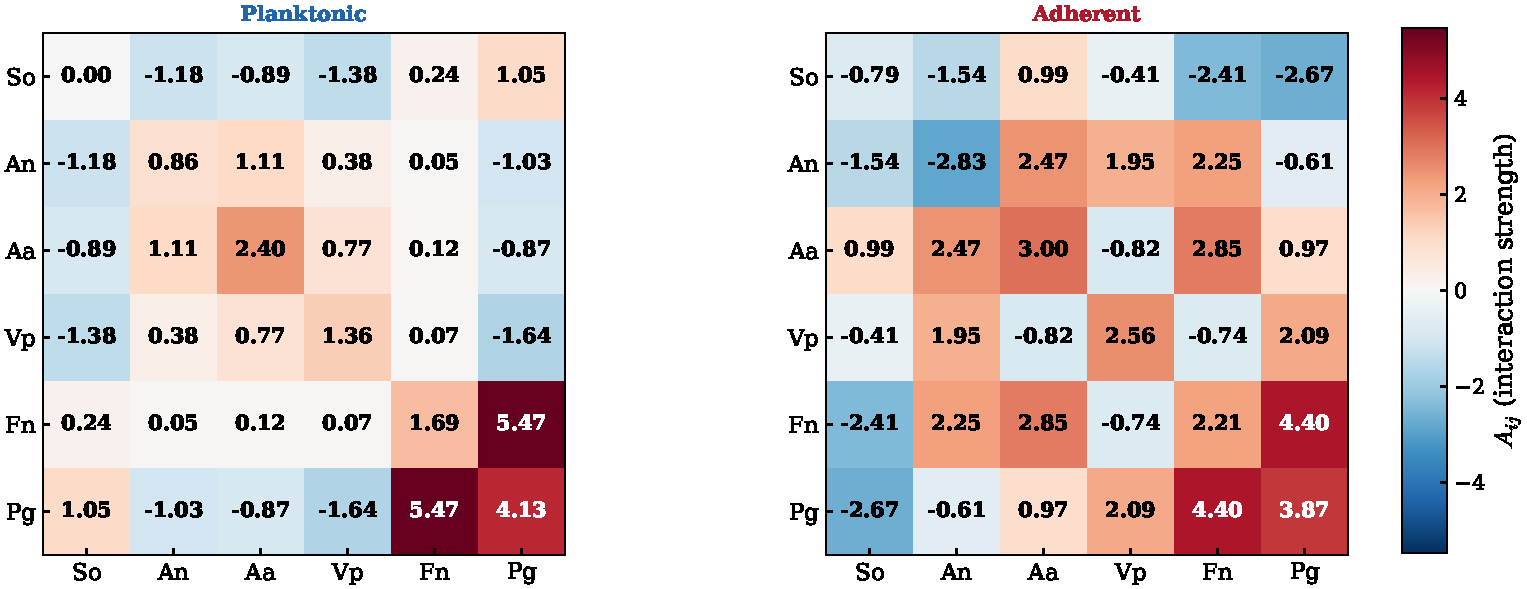
\includegraphics[width=\textwidth]{figures/fig_A_matrix_6sp.pdf}
\caption{MAP interaction matrices $A_{ij}$. Red = mutualistic, blue = competitive.
Both conditions share strong Fn--Pg mutualism ($a_{56} \approx 4$--$6$),
consistent with known coaggregation. Planktonic: So--An mutualism ($a_{12}=3.65$),
So--Vp competition ($a_{14}=-3.70$). Adherent: So--An competition ($a_{12}=-1.54$),
indicating surface attachment fundamentally alters early-colonizer interactions.}
\label{fig:A_matrix}
\end{figure}

\subsection{Interaction Parameter Posteriors}

\begin{figure}[H]\centering
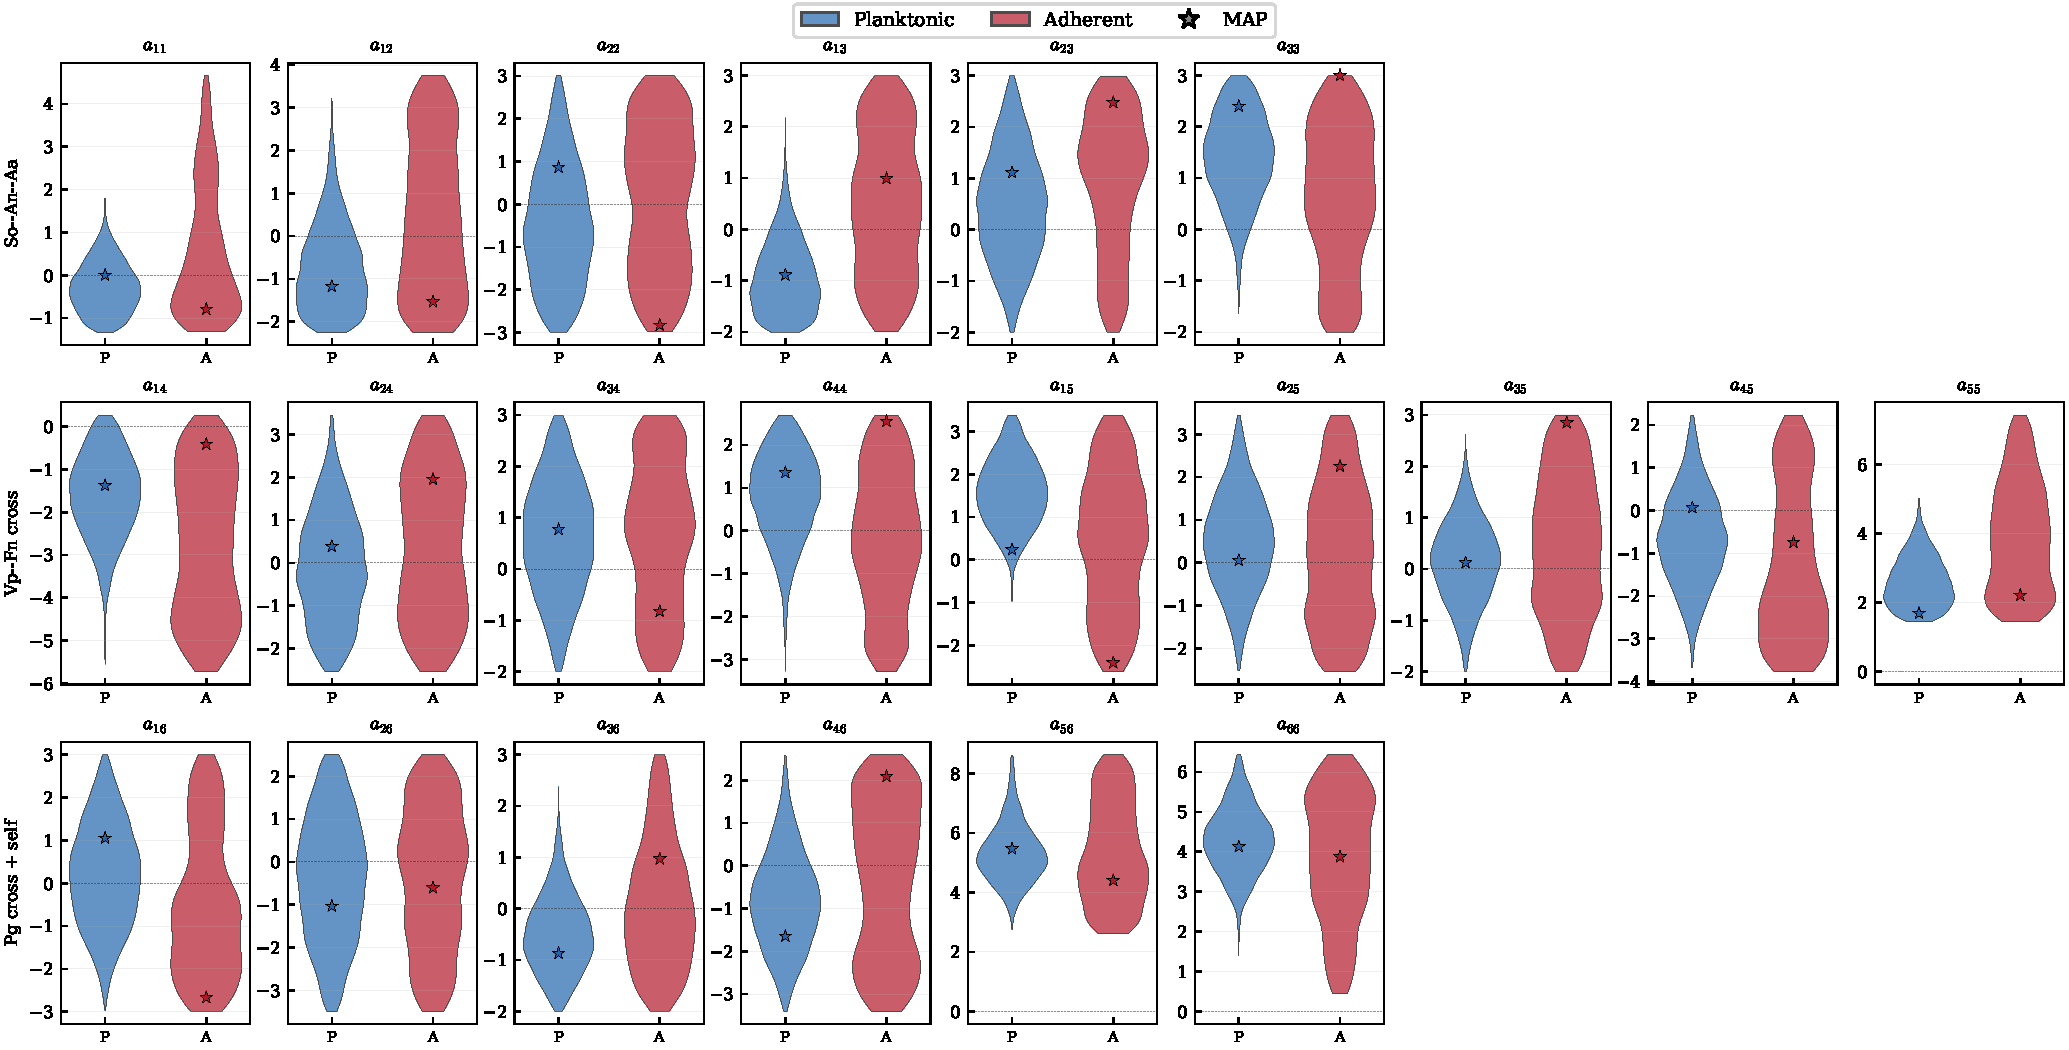
\includegraphics[width=\textwidth]{figures/fig_A_violin_6sp.pdf}
\caption{Posterior distributions of all 21 $a_{ij}$ parameters.
Top: So--An--Aa block. Middle: Vp--Fn cross-interactions. Bottom: Pg.
$a_{56}$ (Fn--Pg) is tightly constrained and positive in both conditions.
Wide posteriors in $a_{14}$, $a_{25}$ indicate partial non-identifiability.}
\label{fig:A_violin}
\end{figure}

\subsection{Growth Rates}

\begin{figure}[H]\centering
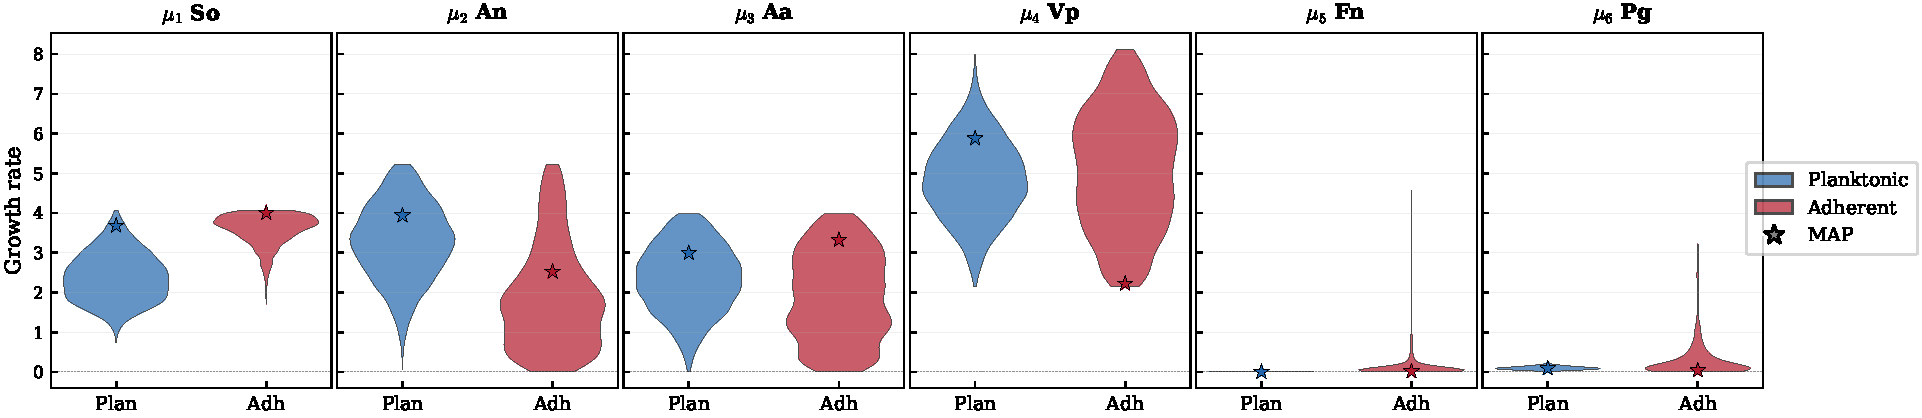
\includegraphics[width=\textwidth]{figures/fig_mu_violin_6sp.pdf}
\caption{Growth rate posteriors. So and Vp have high $\mu$ (fast growers).
Fn and Pg have near-zero $\mu$, relying on interaction terms for dominance.
Aa: $\mu \approx 0$ in planktonic but positive in adherent (surface-adhesion advantage).}
\label{fig:mu_violin}
\end{figure}

\subsection{Observed vs.\ Predicted}

\begin{figure}[H]\centering
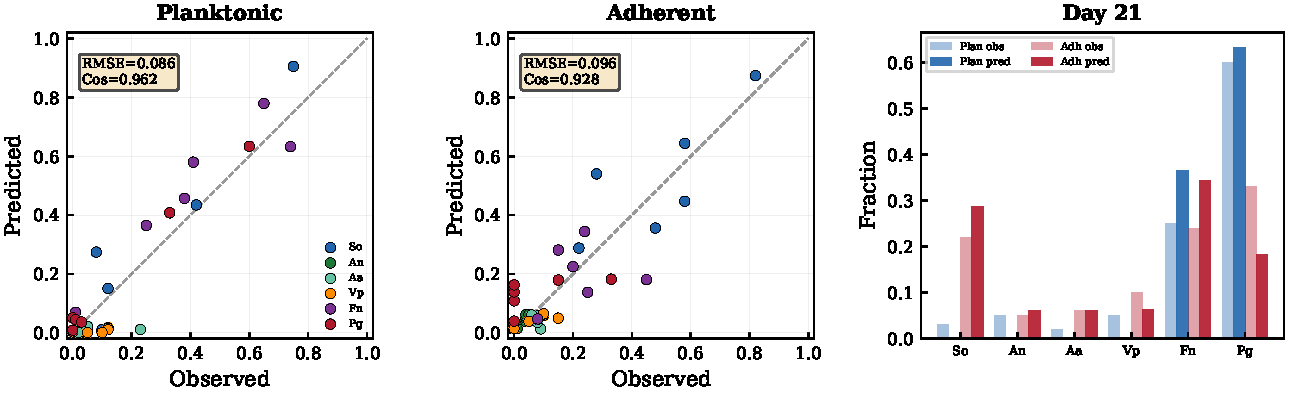
\includegraphics[width=\textwidth]{figures/fig_scatter_day21_6sp.pdf}
\caption{Left/center: obs vs.\ pred scatter (adherent closer to diagonal).
Right: Day~21 equilibrium. Planktonic is Pg-dominated ($\sim$60\%);
adherent is balanced (So/Fn/Pg each $\sim$25--33\%).}
\label{fig:scatter}
\end{figure}

\subsection{Residual Analysis}

\begin{figure}[H]\centering
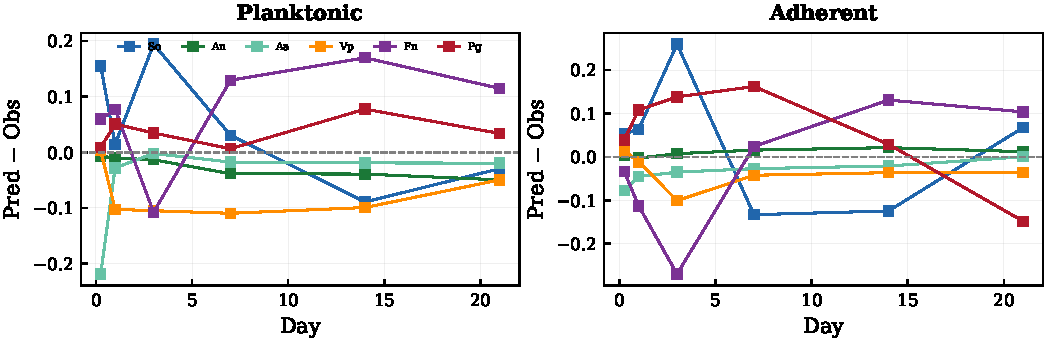
\includegraphics[width=\textwidth]{figures/fig_residuals_6sp.pdf}
\caption{Per-species residuals. Planktonic: largest is Fn Day~3 ($-0.19$)
and Pg Day~14 ($-0.18$). Adherent: So Day~3 ($+0.11$).
All within $\pm 0.20$.}
\label{fig:residuals}
\end{figure}

% ================================================================
\section{Discussion}

\subsection{Model Transferability}

The Hamilton ODE framework, originally calibrated on the Heine 2025 dataset
with 5 species and 4 culture conditions, successfully generalizes to the
Siddiqui 2021 dataset despite substantial differences in experimental design
(Table~\ref{tab:comparison}). The RMSE values of 0.086 (planktonic,
Fig.~\ref{fig:plan_6panel}) and 0.097 (adherent, Fig.~\ref{fig:adh_6panel})
are achieved with the same ODE structure---no additional terms,
compartments, or spatial dimensions were required. This supports the claim
that the Hamilton variational formulation captures fundamental interspecies
dynamics rather than dataset-specific artifacts.

The use of Heine 2025 posterior as an informative prior (shared parameters
$\pm 3.0$) was critical for convergence in the 28-dimensional parameter space.
Without this prior, TMCMC required $>$2 hours for XLA compilation alone and
often converged to degenerate solutions. This hierarchical approach---using
one dataset's posterior as the next dataset's prior---is a natural Bayesian
strategy that could be extended to additional independent datasets as they
become available.

\subsection{Biological Interpretation of Key Parameters}

\textbf{Fn--Pg Hill gate.}
The estimated $K_\mathrm{hill} = 0.115$ (planktonic) indicates that
\textit{P.\ gingivalis} proliferation requires \textit{F.\ nucleatum} abundance
to exceed $\sim$11.5\% of the community---consistent with the observation that
Pg emerges only after Fn has established dominance (Day~7--14). This threshold
is lower than the Heine 2025 estimate ($K = 0.15$), suggesting that the
Siddiqui culture conditions (BHI broth, anaerobic) facilitate earlier
Fn--Pg coaggregation.

\textbf{Planktonic vs.\ adherent interaction reversal.}
The So--An interaction ($a_{12}$, Fig.~\ref{fig:A_matrix}) switches from mutualistic
(+3.65 in planktonic) to competitive ($-1.54$ in adherent). This is biologically plausible:
in bulk medium, both species benefit from shared metabolic byproducts,
while on a surface they compete for limited attachment sites. Similarly,
So--Fn ($a_{15}$) is mildly positive in planktonic but strongly negative
($-2.41$) in adherent, where \textit{F.\ nucleatum}'s bridging role
creates direct spatial competition with early colonizers.

\textbf{Growth rates and interaction trade-off.}
\textit{F.\ nucleatum} and \textit{P.\ gingivalis} have near-zero intrinsic
growth rates ($\mu_5, \mu_6 \approx 0$, Fig.~\ref{fig:mu_violin} and
Table~\ref{tab:map}) in both conditions, achieving dominance entirely through
positive interaction terms. This is consistent with their
ecological strategy as bridging/late colonizers that depend on pre-established
communities rather than rapid autonomous growth.

\subsection{Limitations of the Present Analysis}

\begin{enumerate}
\item \textbf{Observable limitation.} Only $\bar{\varphi}_i = \varphi_i \cdot \psi_i$
is measurable; the decomposition into volume fraction and fitness is
under-determined. The Hamilton variational structure constrains this decomposition
but does not fully resolve it, leading to parameter trade-offs visible in
the wide posteriors of several $a_{ij}$ (Fig.~\ref{fig:A_violin}).

\item \textbf{Single biological replicate.} The Siddiqui data represents $n=1$
biological realization with $n=2$ technical qPCR replicates. The true
between-experiment variability is unknown and likely larger than
$\sigma_\mathrm{obs} = 0.15$.

\item \textbf{Digitization uncertainty.} Composition data were extracted from
published stacked bar charts ($\pm 3$\% precision). Raw qPCR counts would
enable more precise calibration.

\item \textbf{0D assumption.} The ODE assumes a well-mixed system, which is
appropriate for planktonic bacteria but less so for surface-adherent biofilms
where spatial structure, nutrient gradients, and attachment geometry play
significant roles. The Day~7 So recovery in adherent data likely reflects
spatial re-colonization dynamics that cannot be captured by 0D models.

\item \textbf{Planktonic Fn peak.} The model underestimates the Fn peak at Day~3
(74\% observed vs.\ $\sim$55\% MAP, Fig.~\ref{fig:residuals}).
This may require nutrient-coupled dynamics
(Monod kinetics) or time-varying interaction coefficients to fully resolve.
\end{enumerate}

\subsection{Future Directions}

\begin{itemize}
\item \textbf{Monod nutrient coupling}: The \texttt{simulate\_0d\_nutrient} function
already supports well-mixed nutrient dynamics. Adding nutrient competition
could improve Fn peak tracking in planktonic conditions.
\item \textbf{Joint calibration}: Simultaneously fitting planktonic and adherent data
with shared $A_{ij}$ but condition-specific $\mu_i$ would leverage both datasets.
\item \textbf{Additional datasets}: Application to other published in vitro biofilm
succession studies (e.g., The Forsyth Institute, Mark Welch lab CLASI-FISH data)
would further validate transferability.
\item \textbf{Spatial extension}: VEM (Virtual Element Method) or 1D PDE coupling
for adherent biofilm to capture surface-specific dynamics.
\end{itemize}

% ================================================================
\section{MAP Parameter Estimates}

\begin{table}[H]\centering\small
\caption{MAP $\theta$ for planktonic (28 params) and adherent (27 params).}
\label{tab:map}
\begin{tabular}{clccc}
\toprule
Idx & Parameter & Name & Planktonic & Adherent \\
\midrule
    0 & $a_{11}$ & a(So-So)     & +0.003 & -0.791 \\
    1 & $a_{12}$ & a(So-An)     & -1.179 & -1.535 \\
    2 & $a_{22}$ & a(An-An)     & +0.865 & -2.828 \\
    3 & $a_{13}$ & a(So-Aa)     & -0.888 & +0.991 \\
    4 & $a_{23}$ & a(An-Aa)     & +1.108 & +2.474 \\
    5 & $a_{33}$ & a(Aa-Aa)     & +2.400 & +2.998 \\
    6 & $a_{14}$ & a(So-Vp)     & -1.376 & -0.410 \\
    7 & $a_{24}$ & a(An-Vp)     & +0.382 & +1.949 \\
    8 & $a_{34}$ & a(Aa-Vp)     & +0.774 & -0.823 \\
    9 & $a_{44}$ & a(Vp-Vp)     & +1.359 & +2.559 \\
   10 & $a_{15}$ & a(So-Fn)     & +0.235 & -2.409 \\
   11 & $a_{25}$ & a(An-Fn)     & +0.053 & +2.251 \\
   12 & $a_{35}$ & a(Aa-Fn)     & +0.122 & +2.848 \\
   13 & $a_{45}$ & a(Vp-Fn)     & +0.067 & -0.744 \\
   14 & $a_{55}$ & a(Fn-Fn)     & +1.692 & +2.213 \\
   15 & $a_{16}$ & a(So-Pg)     & +1.053 & -2.669 \\
   16 & $a_{26}$ & a(An-Pg)     & -1.033 & -0.609 \\
   17 & $a_{36}$ & a(Aa-Pg)     & -0.869 & +0.969 \\
   18 & $a_{46}$ & a(Vp-Pg)     & -1.644 & +2.089 \\
   19 & $a_{56}$ & a(Fn-Pg)     & +5.468 & +4.404 \\
   20 & $a_{66}$ & a(Pg-Pg)     & +4.129 & +3.874 \\
   21 & $\mu_1$ & $\mu$(So)    & +3.683 & +4.003 \\
   22 & $\mu_2$ & $\mu$(An)    & +3.939 & +2.523 \\
   23 & $\mu_3$ & $\mu$(Aa)    & +2.993 & +3.321 \\
   24 & $\mu_4$ & $\mu$(Vp)    & +5.877 & +2.222 \\
   25 & $\mu_5$ & $\mu$(Fn)    & +0.000 & +0.013 \\
   26 & $\mu_6$ & $\mu$(Pg)    & +0.087 & +0.037 \\
   27 & $K_\mathrm{hill}$ & $K_\mathrm{hill}$ & +0.115 & --- \\
\bottomrule
\end{tabular}
\end{table}

% ================================================================
\section*{References}

\begin{thebibliography}{9}

\bibitem{siddiqui2021}
Siddiqui DA, Fidai AB, Natarajan SG, Rodrigues DC.
Succession of oral bacterial colonizers on dental implant materials:
an in vitro biofilm model.
\textit{Dental Materials} 38(2):384--396, 2022.
DOI: 10.1016/j.dental.2021.12.021.

\bibitem{heine2025}
Heine S, and coauthors.
Multi-species oral biofilm composition under commensal and dysbiotic conditions.
\textit{(Calibration dataset for Hamilton ODE model)}, 2025.

\bibitem{socransky1998}
Socransky SS, Haffajee AD, Cugini MA, Smith C, Kent RL Jr.
Microbial complexes in subgingival plaque.
\textit{J Clin Periodontol} 25(2):134--144, 1998.

\bibitem{hamilton_biofilm}
Hamilton WD.
The genetical evolution of social behaviour.
\textit{J Theor Biol} 7(1):1--16, 1964.

\end{thebibliography}

\end{document}
